%----------------------------------------------------------------------------------------
%	SLIDE 12.
%----------------------------------------------------------------------------------------
\begin{frame}
\frametitle{Parallelisation in physics}
\framesubtitle{In general}

\begin{columns}
	\column{0.38\linewidth}
	{\small
	\begin{itemize}
		\item Running simulation software (e.g. Computer Simulation and Modelling, MSc course -- OpenFoam, GADGET4, HOOMD-blue)
		\item Working on servers (e.g. onco2, tesla, atys, veo1 (known as `kooplex`) etc. at ELTE)
		\item Working on HPC clusters (e.g. ELTE \textit{Atlasz} cluster or the Hungarian Komondor HPC cluster, etc.)
	\end{itemize}}
	
	\column{0.6\linewidth}
	\begin{figure}
		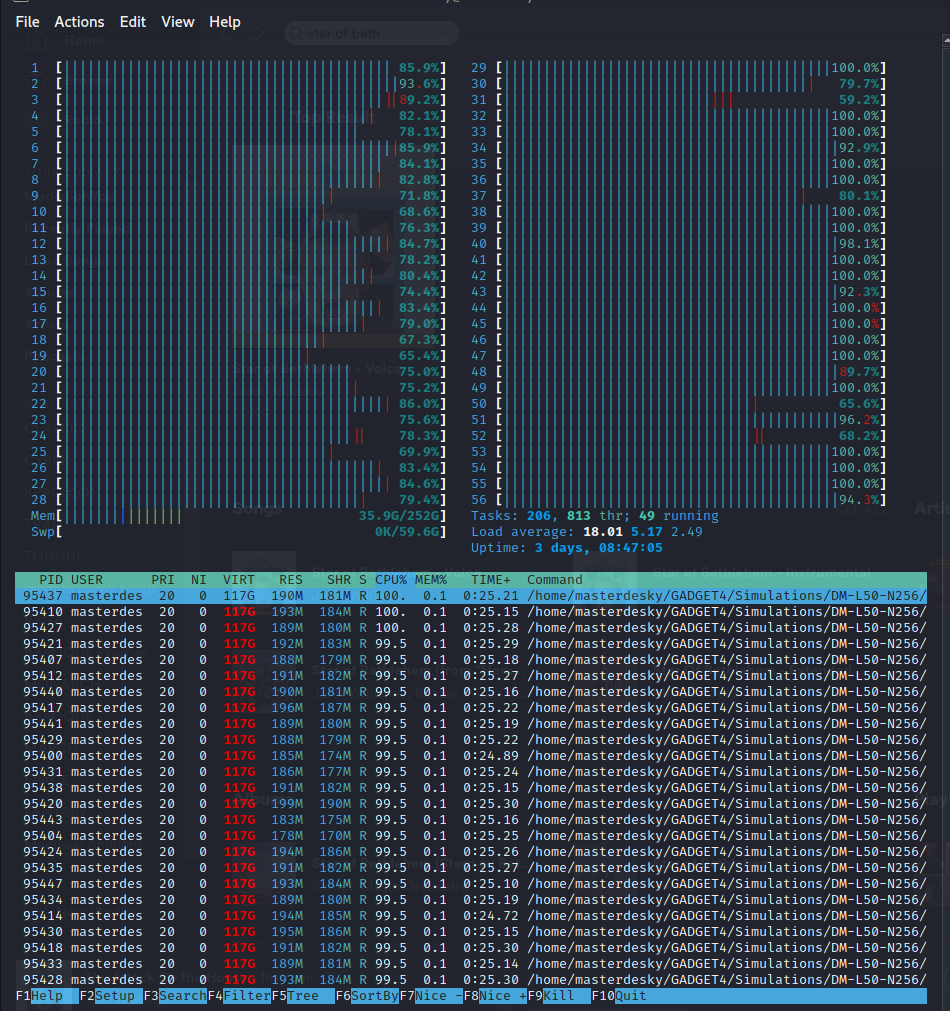
\includegraphics[width=\textwidth]{img/onco2.png}
	\end{figure}

\end{columns}

\end{frame}